\section*{Problem 8}

Compute the inverse Fourier transform of the following signal

\begin{figure}[H]
\caption*{}
\centering
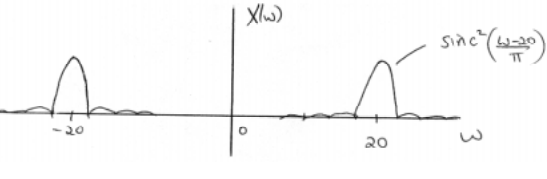
\includegraphics[width=0.8\textwidth]{figs/c2p8.png}
\label{fig:c2p8}
\end{figure} 

\subsection*{Solution}

From the 14th result of the Fourier Transforms table we have:

\begin{equation*}
Tr_\tau(t) =
\begin{cases}
	1 - \frac{|t|}{\tau}  ,& \mbox{if } |t| < \tau \\
	0                     ,& \mbox{if } |t| > \tau
\end{cases}
\end{equation*}

\begin{equation}
\begin{aligned}
\mathfrak{F}\{Tr_\tau(t)\} = \tau \left[ Sa \left( \frac{\omega \tau}{2} \right) \right]^2 \\
\mathfrak{F}\{Tr_2(t)\} = 2 Sa(\omega)^2 
\label{eq:c2p5}
\end{aligned}
\end{equation} 

First, we transform sinc into a known function like Sa: 
\begin{equation*}
\begin{aligned}
sinc^2 \left( \frac{\omega}{\pi} \right) = Sa^2(\omega)
\end{aligned}
\end{equation*} 

As we saw in Point 4, when we multiply by a $\cos$ in time 
we are adding 2 components of the function displaced simetrically
with half of its amplitude. The displacement in the plot is
of 20, therefore we need to multiply by a $\cos(20t)$.
We end up having:

\begin{equation*}
x(t) = Tr_2(t) \cos(20t)
\end{equation*} 
